%The polygraph is a matrix, which is rotated by -45°. We pre-rotate the labels by 45° so that they end up right in the end.
% paths use numerical coordinates rather than labels since the effects are different for unclear reasons

\begin{turn}{-45}
 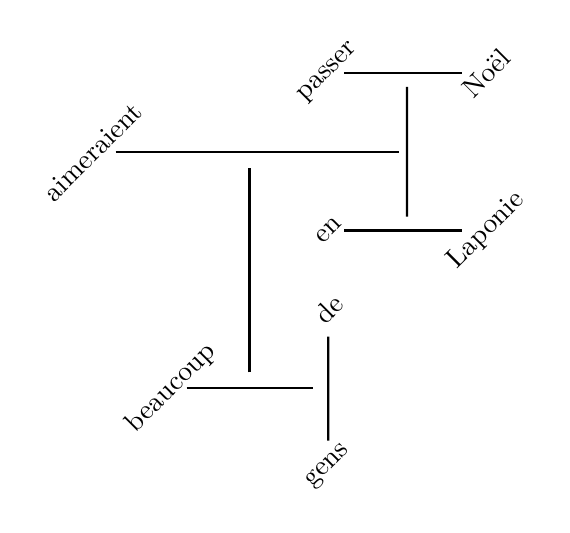
\begin{tikzpicture}
\node (passer)   at (4,5)  [rotate=45] {passer};
\node (b)   at (5,5)  [rotate=45] {};
\node (Noël)   at (6,5)  [rotate=45] {Noël};
%
\node (aimeraient)   at (1,4)  [rotate=45] {aimeraient};
\node (x)   at (3,4)  [rotate=45] {};
\node (y)   at (5,4)  [rotate=45] {};
%
\node (en)   at (4,3)  [rotate=45] {en};
\node (a)   at (5,3)  [rotate=45] {};
\node (Laponie)   at (6,3)  [rotate=45] {Laponie};
%
\node (de)   at (4,2)  [rotate=45] {de};
%
\node (beaucoup)   at (2,1)  [rotate=45] {beaucoup};
\node (z)   at (3,1)  [rotate=45] {};
\node (c)   at (4,1)  [rotate=45] {};

%
\node (gens)   at (4,0)   [rotate=45]  {gens};
%
\draw[thick,shorten <=2mm, shorten >=3mm] (4,5) -- (6,5);
\draw[thick,shorten <=3mm, shorten >=1mm] (1,4) -- (5,4);
\draw[thick,shorten <=2mm, shorten >=3mm] (4,3) -- (6,3);
% 2
\draw[thick,shorten <=2mm, shorten >=2mm] (2,1) -- (4,1);

%
% \draw[thick] (z) -- (x);
\draw[thick,shorten <=2mm, shorten >=2mm] (3,1) -- (3,4);
\draw[thick] (gens) -- (de);
\draw[thick] (a) -- (b);
\end{tikzpicture}
\end{turn}
